\section{How the sine and self-power circuits compute their outputs}
\label{app:smooth-circuits}

\paragraph{Circuits and reference values.}
We designed one circuit for the sine of a scalar input $x$ in radians on $[-16,16]$ and one for the self-power function $x\mapsto x^x$ on $[0,128]$, setting $0^0=1$ by continuity. Each design uses the formula and its domain. In this engineered weight-space programming (WSP) condition, we set the weights of each graph before evaluating any test input. The circuit is a directed acyclic graph, meaning a list of operations in which each result depends only on earlier operations. Its operations are scalar affine maps (weighted sums plus offsets) and rectified linear units, $\relu(v)=\max(0,v)$ for scalar $v$. We checked that at least one argument of every multiplication depends only on fixed coefficients. The graph uses separate binary64 operations, each rounded to nearest with ties to even. This fixes the order of addition and multiplication and permits subnormal results, the values spaced $2^{-1074}$ apart below the smallest positive normal number $2^{-1022}$.

Our mathematical reference is the exact function rounded once to binary64. We computed it with GNU MPFR version 4.2.2, a multiple-precision library with correctly rounded elementary functions~\cite{mpfr}, at 53 significant bits and cross-checked challenge values by rounding higher-precision evaluations. NumPy, the numerical library used in the earlier tests, differs from MPFR on 321 of the 8,192 ordinary outer sine inputs and 3 of the 4,096 ordinary outer self-power inputs. Here an exact match means agreement with MPFR. For the unit-in-the-last-place (ULP) distance we count representable steps between prediction and reference, identifying signed zeros.

\paragraph{Choosing a bit using rectified linear units.}
Let $r$ be a nonnegative binary64 remainder, $k$ an integer exponent used by the circuit and $a=2^k$ a normal threshold. Its nearest smaller binary64 value is $a-2^{k-53}$. Define the threshold gate
\[
 B_k(r)=\relu\!\left(1-\relu\!\left(2^{53-k}(a-r)\right)\right).
\]
At $r\ge a$ the inner rectifier returns zero. At $r<a$ the gain $2^{53-k}$ scales the difference to at least one. Thus the output is precisely the bit for the decision $r\ge a$. To copy a signed value $v$ only when a bit $b$ equals one, choose a bound $M\ge |v|$ and evaluate $\relu(v-M(1-b))-\relu(-v-M(1-b))$. The result is $v$ when enabled and zero otherwise. The circuit uses these operations to select terms of known sums. Its two-word variant represents an intermediate by the sum of a leading binary64 value and a smaller correction. Compensated arithmetic retains part of the rounding error of each sum or constant product in that correction~\cite{dekker1971}.

\paragraph{Sine.}
Starting with angle zero, we store its sine and cosine, zero and one. We inspect the powers $2^k$ in $|x|$ from $k=4$ downward. Whenever $B_k$ selects a power, we subtract it from the remainder and apply the sine and cosine angle-addition formulas for a rotation of $2^k$ radians. Its sine and cosine are coefficients computed before inference by Taylor series for angles up to one radian and angle doubling for larger angles. The 83-stage graph ends at $k=-78$ and restores the sign of $x$. For $|x|\le 2^{-26}$ it returns $x$ directly, because the bound $|x-\sin x|\le |x|^3/6$ is below half the distance to the next binary64 value toward zero.

\paragraph{Self-power.}
For $x\ge 2^{-64}$, choose an integer exponent $e$ and fractional remainder $u$ with $x=2^e(1+u)$ and $0\le u\le 1$. Write $\log$ for the natural logarithm. At fractional digit $j$, starting at $j=1$, let $d=2^{-j}$. When the leading word of $u$ reaches $d$, multiply $u-d$ by the stored coefficient $1/(1+d)$ and add the stored $\log(1+d)$ to a running logarithm initialized at $e\log 2$. The identity $(1+u)/(1+d)=1+(u-d)/(1+d)$ explains the update. After the last digit, add the remaining $u$ as a first-order approximation to $\log(1+u)$. Next form $y=1+x\log x$ by adding scaled copies of that logarithm for the selected input bits. Finally, start at $\exp(-1)$, where $\exp$ is the natural exponential, and multiply by the stored $\exp(2^k)$ for each selected bit of $y$. The exact-arithmetic identity is $\exp(-1)\exp(y)=x^x$. For $x<2^{-64}$ the circuit returns one. These digitwise logarithm and exponential methods have precedents in elementary-function algorithms \href{https://doi.org/10.1109/12.295857}{(Bajard, Kla and Muller, 1994)}.

\paragraph{Comparing sizes.}
We count separately a stored coefficient, an occurrence of a coefficient in an expanded affine operation, and an executed rectifier. The engineered WSP graphs for 83-stage sine and 84-fractional-bit self-power store 500 and 1,352 coefficient words. Each word overwrites a scalar Xavier draw, uniform on $[-\sqrt{3},\sqrt{3}]$. The topology and fixed signs already encode the algorithm. Expanding repeated coefficient uses gives 25,395 and 35,908 affine occurrences and 1,506 and 2,618 rectifiers. The affine count charges two coefficients for a sum of two variables or a variable plus an offset and one for scaling. The stored graphs also have four and seven fixed structural constants respectively. Figure~\ref{fig:smooth-relu} identifies the first tested sizes to pass the ordinary outer samples. Smaller unswept graphs could have the same accuracy.

\begin{figure}[htbp]
\centering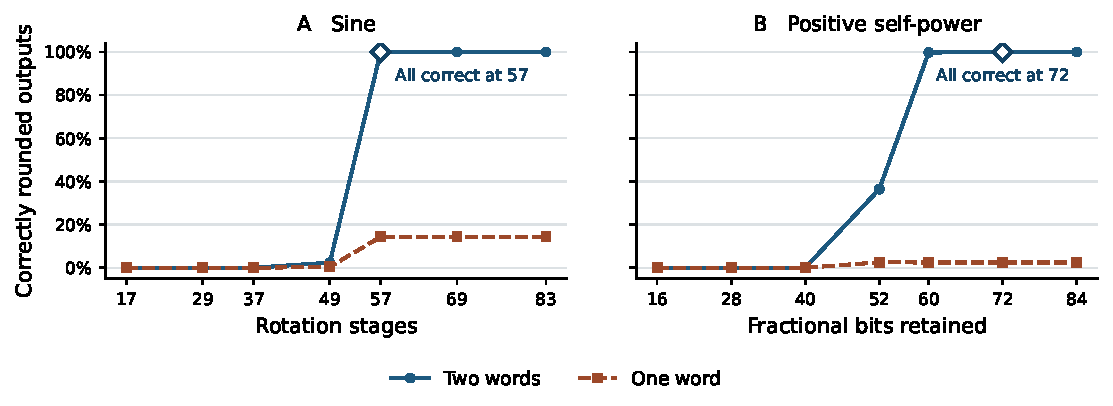
\includegraphics[width=.97\linewidth]{smooth_precision.pdf}
\caption{Fraction of inputs for which the network returns the correctly rounded mathematical value. The sine panel pools 4,096 inputs from each of $[-10,-3]$ and $[3,10]$. The self-power panel uses 4,096 inputs from $[3,10]$. Each curve evaluates the same inputs at seven sizes. The solid curve stores a leading word plus a rounding correction, and the dashed curve uses one word per intermediate. An open diamond marks the first sampled size with no misses in each panel. At 60 fractional bits, the two-word self-power circuit still misses 10 of 4,096 inputs.}
\label{fig:smooth-relu}
\end{figure}

\paragraph{Where agreement fails.}
At 57 sine stages (344 stored words) and 72 fractional bits for self-power (1,208 words), the two-word circuits first matched their respective full ordinary outer samples. The two largest WSP circuits also matched all 4,096 central and 32,768 independently drawn outer inputs per task, plus 8,192 inputs per task with exponents sampled uniformly into the subnormal range. Both had zero raw root mean squared error (RMSE) on the ordinary central and outer sets. Sine matched 102 values near nonzero multiples of $\pi$ (half a turn in radians) and 4,096 farther inputs in $[10,16]$. Self-power matched 213 values at or adjacent to powers of two and 4,096 farther inputs in $[10,128]$.

CORE-MATH is a public project that distributes inputs whose function values are hard to round correctly. On its sine inputs the largest graph misses 12 of 30,326 distinct values in $[-16,16]$, including one of 1,884 in the requested outer intervals. Each miss is one representable step. Across all 30,326 hard inputs the RMSE is $7.31\times10^{-19}$, and on the 1,884 hard outer inputs it is $2.50\times10^{-21}$. We write inputs as hexadecimal significands times powers of two, with \texttt{p} introducing the base-two exponent. At $x=\texttt{0x1.9239c4bbb44a4p+1}$ the absolute error is $1.08\times10^{-19}$ and the absolute error divided by $|\sin x|$ is $1.36\times10^{-16}$. The archive records the source revision and file hash for the \href{https://core-math.gitlabpages.inria.fr/worst.html}{public input corpus}.

For self-power, values just below one are spaced $2^{-53}$ apart. For integers $j=0,\ldots,127$, we located the small positive input satisfying $x\log x=\log(1-(j+1/2)2^{-53})$. Its exact output is a midpoint between two binary64 values. We tested the closest binary64 input and its three neighbors on either side. Of 896 outputs, 446 matched and the remaining 450 were one step away. At $x=\texttt{0x1.8e2e5fb51604cp-60}$ the network returns one. The reference is the next value below one, an absolute difference of $2^{-53}$. The RMSE across the 896 near-midpoint inputs is $7.87\times10^{-17}$.

\paragraph{Gradient and product-gate controls.}
On the same 83-stage sine graph, we trained all 500 slots with adaptive moment estimation (Adam), using gradients propagated backward from the loss. We gave the optimizer 1,024 central labels, three independent Xavier starts, 100 updates at learning rate $0.01$ and 32 observations per update. Respectively two, two and zero slots changed, and each run matched zero outer outputs exactly. Outer RMSE in seed order was 16.51, 8.14 and 15.96, compared with zero for the same WSP graph. A separate comparison allowed products of two input-dependent values. We fitted a degree-65 odd polynomial by full-batch Gauss--Newton updates (least-squares updates to the locally linear predictions) in a Chebyshev basis (polynomials orthogonal on a rescaled central interval under the Chebyshev weight). We evaluated both this fit and the formula-written Taylor coefficients with Horner's rule, which alternates multiplication by the argument with addition of a coefficient. Using two words for each of its 33 odd-power coefficients, the formula-written network matched all 8,192 ordinary outer sine values but missed 68 of the 102 probes near roots. The central-label fit matched none of the 8,192 and had outer RMSE $1.13\times10^{35}$, compared with zero for the Taylor coefficients. The electronic tables in \path{revision/numeric_metrics/} retain raw RMSE and exact counts for each size, split and fitted control.
